\documentclass[usepdftitlre=false, debug]{beamer}

\usepackage[francais]{babel}
\usepackage[T1]{fontenc}
\usepackage[ansinew]{inputenc}
\usepackage{lmodern}
\usepackage{graphicx}
\usepackage{listings}
\usepackage{color}
\usepackage{pgf}
\usepackage{tikz}
\usetikzlibrary{arrows,automata}



%%%%%%%%%%%%%%%%%%%%%%%%%%%%%%%%%%%%%%%%%%%%%%%%%%%%%%%%%%%%%%%%%%%%%%%%%%%%%%%%%%%%%%%%%%%%%%%%
\usetheme{Rochester}
\usecolortheme{default}

\title{WinEchek}
\author{Mathis Deloge, Antoine Petot, Ange Picard, Arthur Carchi, Lucas Fougerouse, Vincent Dereclenne}
\institute{IUT Informatique Dijon / Auxerre}
\date{Lundi 14 Novembre 2016}
%%%%%%%%%%%%%%%%%%%%%%%%%%%%%%%%%%%%%%%%%%%%%%%%%%%%%%%%%%%%%%%%%%%%%%%%%%%%%%%%%%%%%%%%%%%%%%%%



\definecolor{mygreen}{rgb}{0,0.6,0}
\definecolor{mygray}{rgb}{0.5,0.5,0.5}
\definecolor{mymauve}{rgb}{1,0,0}

\lstset{ %
  backgroundcolor=\color{gray!30!white},   % choose the background color
  basicstyle=\small\ttfamily,        % size of fonts used for the code
  breaklines=true,                 % automatic line breaking only at whitespace
  captionpos=b,                    % sets the caption-position to bottom
  commentstyle=\color{mygreen},    % comment style
  escapeinside={\%*}{*)},          % if you want to add LaTeX within your code
  keywordstyle=\color{blue},       % keyword style
  stringstyle=\color{mymauve},     % string literal style
	numbers=left,
	frame=leftline,
	xleftmargin=42pt
}

\setbeamertemplate{navigation symbols}{%
\insertbackfindforwardnavigationsymbol
}

\setbeamercolor{background canvas}{bg=yellow!10!white}

\AtBeginSubsection[]
{
  \begin{frame}
  \frametitle{Sommaire}
  \small \tableofcontents[currentsection, currentsubsection]
  \end{frame}
}

\begin{document}

\begin{frame}
	\titlepage
\end{frame}

\section{WinEchek}
\begin{frame}
	\frametitle{WinEchek}
	\begin{block}{Rappel des enjeux}
	\begin{itemize}
	 \item D�velopper une application de jeu d'�chec afin de permettre une mont�e en connaissance, notament avec le langage C\#, aborder les intelligence artificelles et la gestion du r�seau.
	 \item Arriver � pr�senter un livrable final conforme aux attentes de d�but de projet.
	 \item R�aliser et suivre un projet d'ampleur moyenne sur plusieurs mois.
	\end{itemize}
	\end{block}

\end{frame}

\begin{frame}
	\frametitle{WinEchek}
	\begin{block}{Description du projet}
	Un jeu d'�chec permettant de :
	\begin{itemize}
	 \item Jouer en local contre un autre joueur
	 \item Jouer en local contre une intelligence artificielle
	 \item Jouer en r�seau contre un autre joueur
	\end{itemize}

	\end{block}
\end{frame}

\section{Backlog Produit}
\subsection{Rappel du Backlog}
\begin{frame}
	\frametitle{Rappel du Backlog}
	  \begin{itemize}
	  \item Jouer sur la m�me machine
	    \begin{itemize}
	      \item {\textcolor{orange}{Moyenne}} Afficher quel joueur doit jouer
	    \end{itemize}
	  \item G�rer la partie
	    \begin{itemize}
	      \item {\textcolor{orange}{Moyenne}} Annuler un coup
	      \item {\textcolor{orange}{Moyenne}} Rejouer un coup
	      \item {\textcolor{orange}{Moyenne}} Afficher l'historique
	      \item {\textcolor{green}{Basse}} Afficher les pi�ces prises
	      \item {\textcolor{green}{Basse}} Afficher le nombre de tours
	      \item {\textcolor{green}{Basse}} Afficher le timer
	      \item {\textcolor{red}{Haute}} Sauvegarder une partie
	      \item {\textcolor{red}{Haute}} Charger une partie
	    \end{itemize}
	  \item Jouer un tour
	    \begin{itemize}
	      \item {\textcolor{red}{Haute}} D�placer une pi�ce
	      \item {\textcolor{orange}{Moyenne}} Afficher les d�placements possibles
	      \item {\textcolor{red}{Haute}} Promouvoir une pi�ce
	      \item {\textcolor{red}{Haute}} Prendre une pi�ce
	      \item {\textcolor{red}{Haute}} Roquer
	    \end{itemize}
	  \end{itemize}
\end{frame}


\subsection{Avanc�es Backlog}
\begin{frame}
	\frametitle{Avanc�es Backlog}
	  \begin{itemize}
	  %\item Jouer sur la m�me machine
	  %  \begin{itemize}
	  %    \item {\textcolor{orange}{Moyenne}} Afficher quel joueur doit jouer
	  %  \end{itemize}
	  \item G�rer la partie
	    \begin{itemize}
	      \item {\textcolor{orange}{Moyenne}} Annuler un coup
	      \item {\textcolor{orange}{Moyenne}} Rejouer un coup
	      \item {\textcolor{orange}{Moyenne}} Afficher l'historique
	  %    \item {\textcolor{green}{Basse}} Afficher les pi�ces prises
	  %    \item {\textcolor{green}{Basse}} Afficher le nombre de tours
	  %    \item {\textcolor{green}{Basse}} Afficher le timer
	      \item {\textcolor{red}{Haute}} Sauvegarder une partie
	      \item {\textcolor{red}{Haute}} Charger une partie
	    \end{itemize}
	  \item Jouer un tour
	    \begin{itemize}
	      \item {\textcolor{red}{Haute}} D�placer une pi�ce
	      \item {\textcolor{orange}{Moyenne}} Afficher les d�placements possibles
	  %    \item {\textcolor{red}{Haute}} Promouvoir une pi�ce
	      \item {\textcolor{red}{Haute}} Prendre une pi�ce
	  %    \item {\textcolor{red}{Haute}} Roquer
	    \end{itemize}
	  \end{itemize}
\end{frame}


\section{Interface graphique}
\begin{frame}
	\frametitle{Interface graphique}
	\begin{block}{GUI}
		\begin{itemize}
		 \item Application responsive
		 \item Couleur de l'application
		 \item Menu des options de partie
		 \item Historique des coups
		 \item Acc�s au git
		 \item Affichage d'un plateau de jeu
		 \item Affichage de pi�ce sur le plateau de jeu
		\end{itemize}
	\end{block}
\end{frame}

\subsection{Historique des coups}
\begin{frame}
	\frametitle{Historique des coups}
	\begin{center}
	 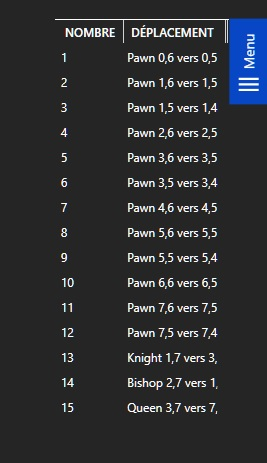
\includegraphics[width=4cm]{Images/Historique.jpg}
	\end{center}
\end{frame}



\subsection{Affichage du plateau et des pi�ces}
\begin{frame}
	\frametitle{Affichage du plateau et des pi�ces}
	\begin{center}
	 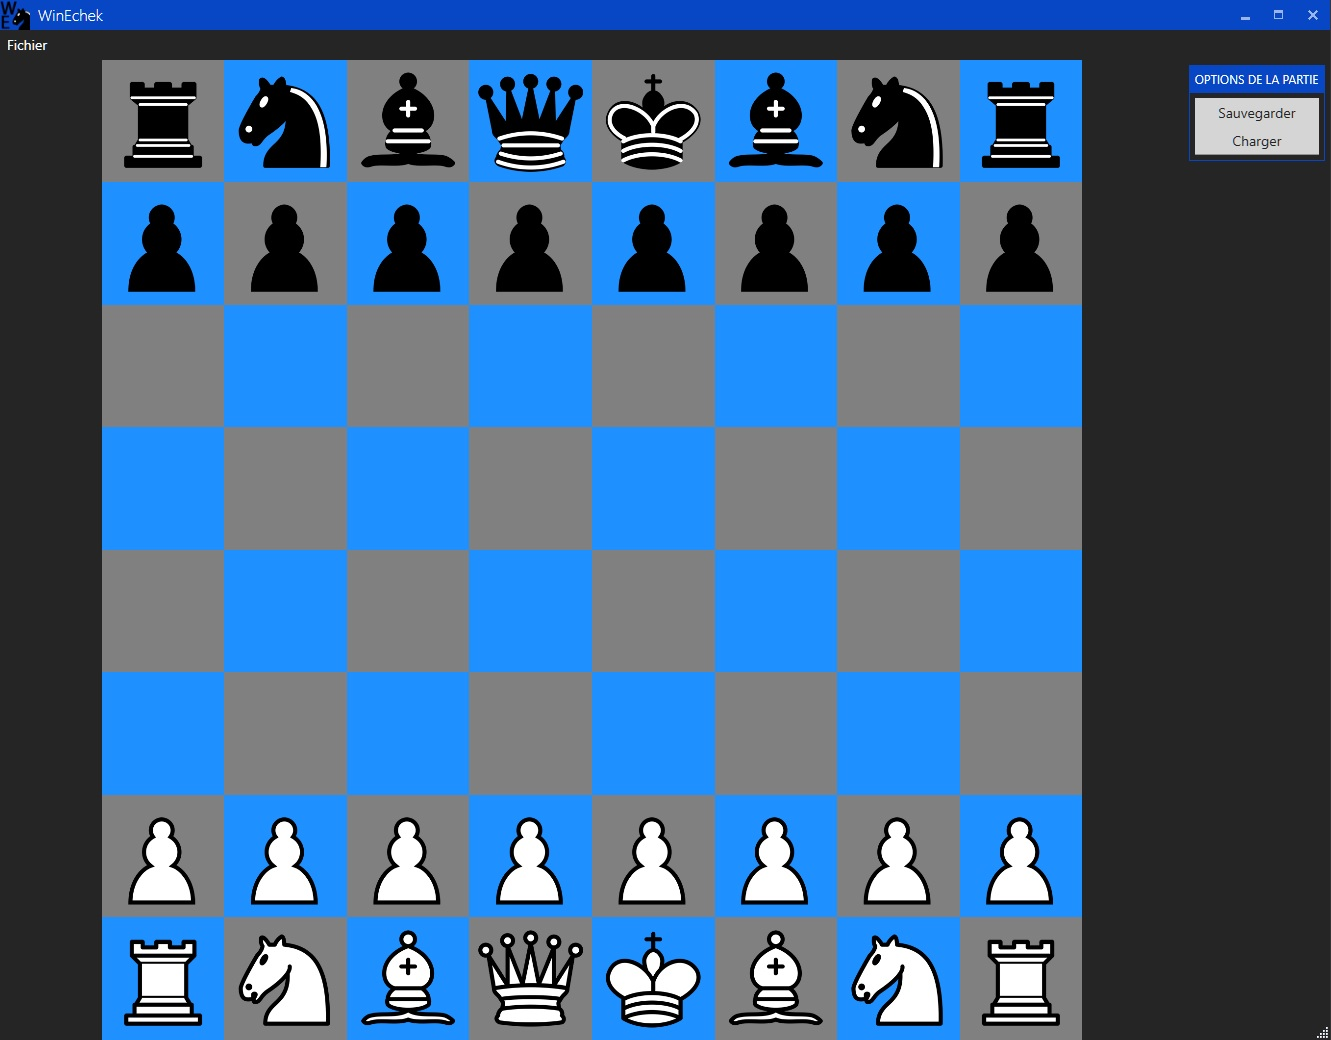
\includegraphics[width=11cm]{Images/board1.jpg}
	\end{center}
\end{frame}


\section{Logique de jeu}
\subsection{D�placer une pi�ce}
\begin{frame}
	\frametitle{D�placer une pi�ce}
	\begin{center}
	 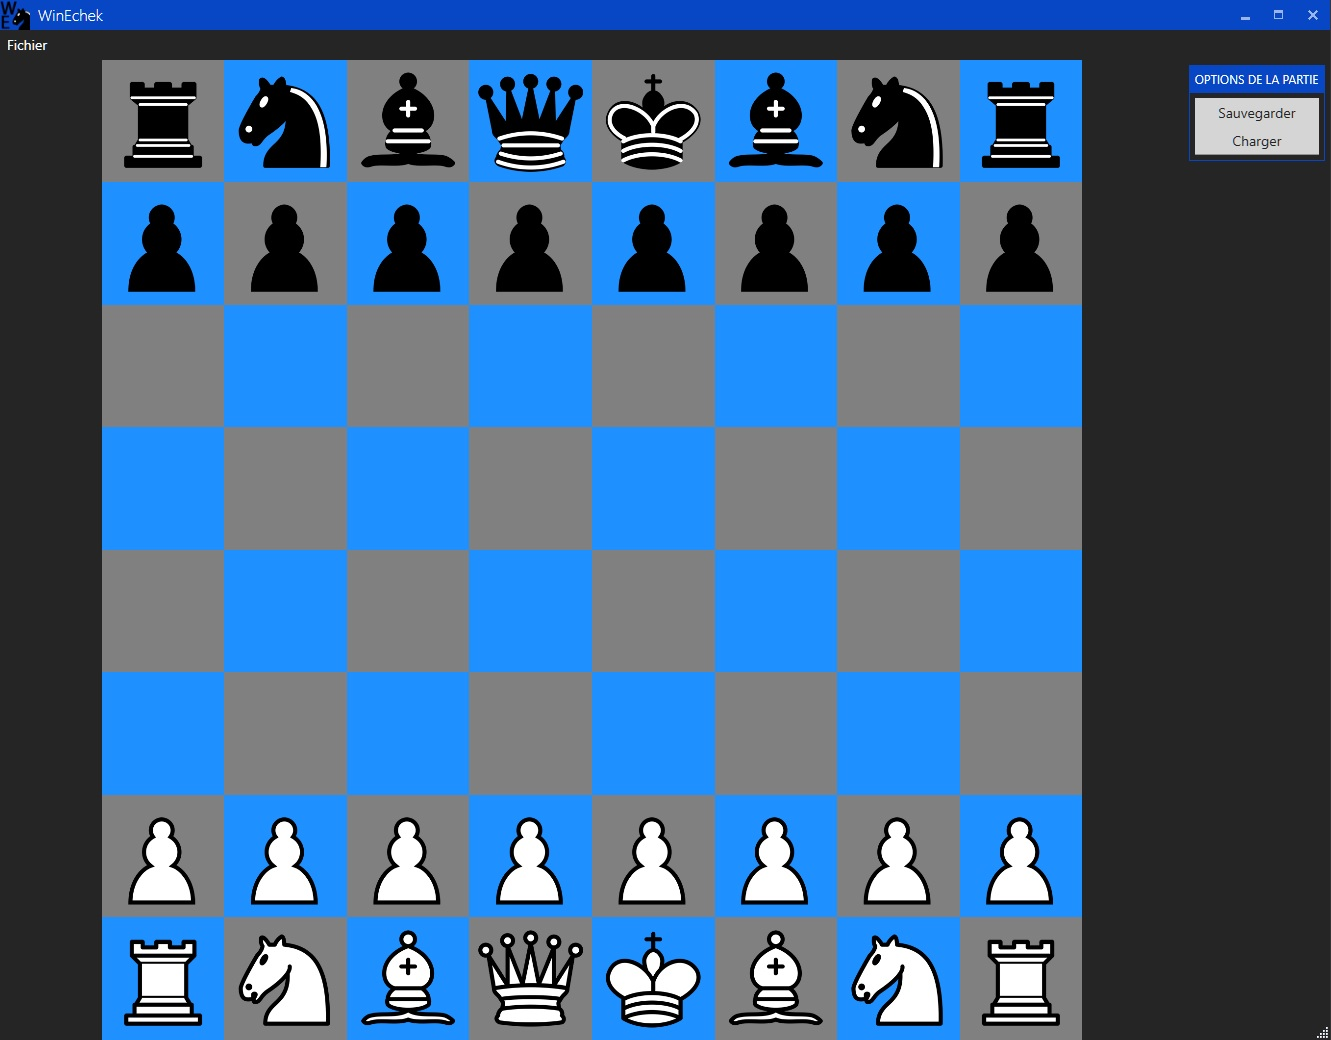
\includegraphics[width=11cm]{Images/board1.jpg}
	\end{center}
\end{frame}




\subsection{Prendre une pi�ce}
\begin{frame}
	\frametitle{Prendre une pi�ce}
	\begin{center}
	 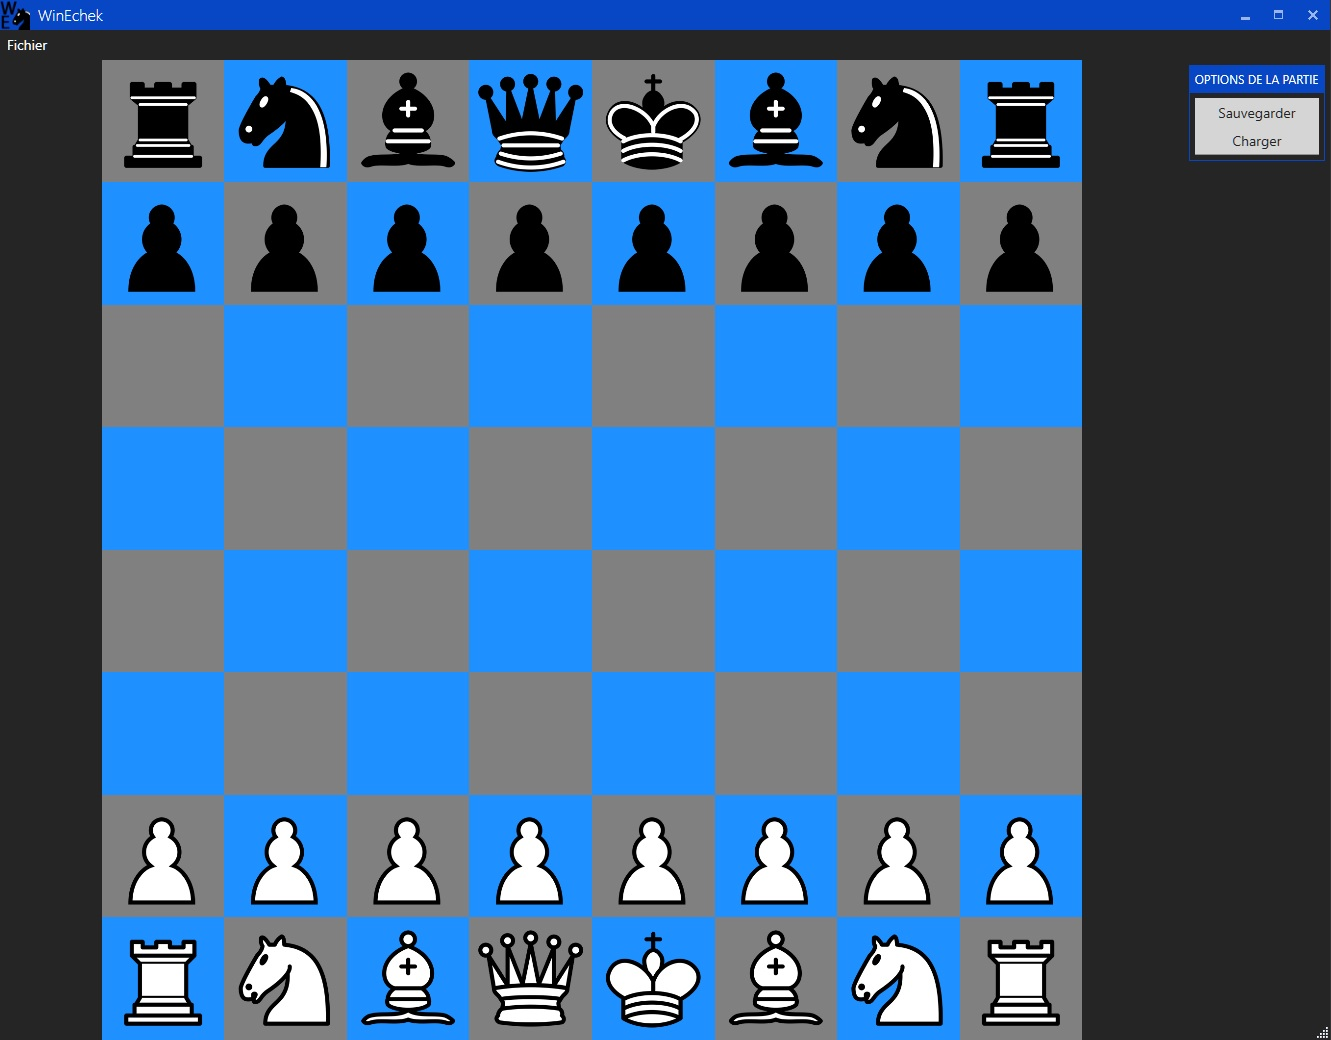
\includegraphics[width=11cm]{Images/board1.jpg}
	\end{center}
\end{frame}






\section{Pour la suite...}
\begin{frame}
	\frametitle{Pour la suite...}
	\begin{center}
	D�finissons ensemble le prochain sprint !
	\end{center}
\end{frame}

\begin{frame}
  \frametitle{Sommaire}
  \tableofcontents
\end{frame}

\end{document}